\begin{frame}[fragile]
  \frametitle{Tabelle Semplici - 3}
  
  Analizziamo quanto visto
  \vspace{1em}
  \begin{itemize}
   \item<1-> Si inizia il blocco come per l'elenco puntato, con il comando \inline{\begin{table}[]}.
   \item<2->Nelle parentesi quadre si specifica la posizione della tabella rispetto al testo.
   \item<3->In questo caso [h!] posiziona la tabella dove l'abbiamo scritta.
   \item<4->Ci sono altre posizioni nelle quali \`e possibile inserire la tabella.
   \item<5-> Centriamo la tabella con \mintinline{latex}{\centering}
   \item<6->\mintinline{latex}{\caption{}} permette di inserire una didascalia sotto la tabella    
  \end{itemize}
  
  \begin{textblock*}{5cm}(8.4cm,1.4cm)
   
\includegraphics[scale=0.07]{lens}
  \end{textblock*}

\end{frame}


\begin{frame}
  \frametitle{Tabelle Semplici - 4}
  Queste sono tutte le possibili posizioni nelle quali possiamo creare la tabella:
  
\begin{table}[h!]
\centering
\begin{tabular}{l|l}
\hline
h      & Posiziona la tabella dove l'abbiamo scritta \\ \hline
t        & Posiziona la tabella in alto nella pagina \\ \hline
b    & Posiziona la tabella in basso nella pagina \\ \hline
p         & Inserisce la tabella in una pagina dedicata  \\ \hline
H  & Posiziona la tabella precisamente (equivalente di h!) \\ \hline
\end{tabular}
\caption{Posizioni delle Tabelle}
\end{table}
Accanto ad ognuno di questi elementi possiamo inserire il !\\
Questo comando \underline{impone} che la tabella venga messa precisamente nel punto in cui viene inserito il comando. Infatti, senza il punto esclamativo, \LaTeX{} posiziona la tabella nel punto specificato solo se ritiene che sia conforme ai parametri.
\end{frame}

\begin{frame}
  \frametitle{Tabelle Semplici - 6}
  Se la tabella \underline{non} richiede di poter occupare tutto lo spazio a disposizione, \`e possibile inserire del testo prima o dopo questa, grazie al pacchetto \textbf{wrapfig}.
  
\begin{esempio}{Una tabella con testo a lato}
\begin{code}
\inputminted[linenos, fontsize=\footnotesize] {latex} {res/examples/tabellaWrapped1.tex}
\end{code}
\end{esempio}

\end{frame}

\begin{frame}
  \frametitle{Tabelle Semplici - 6}
  \begin{code}
\inputminted[linenos, fontsize=\footnotesize] {latex} {res/examples/tabellaWrapped2.tex}
\end{code}
  
\end{frame}

\begin{frame}
  \frametitle{Tabelle Semplici - 6}
  Il risultato \`e il seguente:
   \centering
   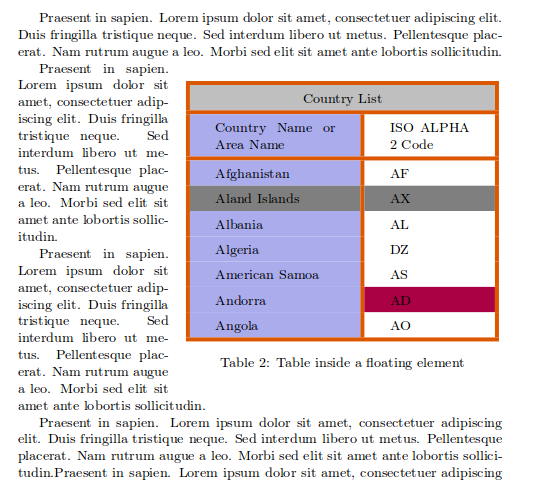
\includegraphics[scale=0.4]{PositioningTable}
\end{frame}